\documentclass[tikz,border=10pt]{standalone}
\begin{document}
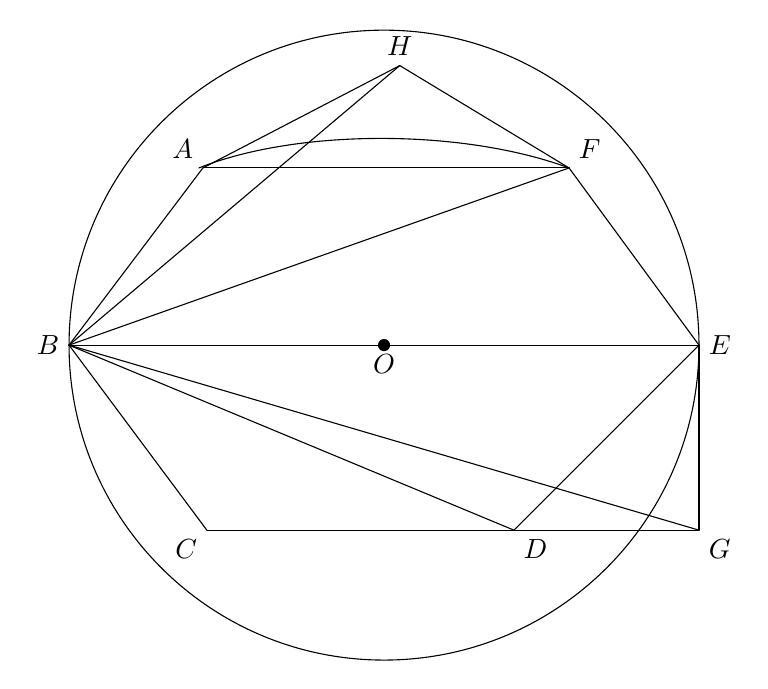
\begin{tikzpicture}[line cap=round,line join=round,scale=1]

% Coordinates
\coordinate (O) at (0,0);
\coordinate (B) at (-4,0);
\coordinate (E) at (4,0);

\coordinate (A) at (-2.3,2.25);
\coordinate (F) at (2.35,2.25);
\coordinate (C) at (-2.25,-2.35);
\coordinate (D) at (1.65,-2.35);

\coordinate (H) at (0.2,3.55);
\coordinate (G) at (4,-2.35);

% Circle
\draw (O) circle (4);

% Chords / segments on the circle
\draw (B)--(E);
\draw (A)--(F);
\draw (C)--(D);

% Polygonal / interior segments
\draw (B)--(A);
\draw (B)--(C);
\draw (B)--(F);
\draw (B)--(D);
\draw (B)--(H);
\draw (D)--(E);
\draw (E)--(F);

% Exterior triangle/rectangle-like parts
\draw (H)--(A);
\draw (H)--(F);
\draw (E)--(G);
\draw (D)--(G);
\draw (B)--(G);

% Upper arc-like curve shown inside the top
\draw (-2.35,2.25) .. controls (-1.1,2.75) and (1.0,2.75) .. (2.35,2.25);

% Point O
\fill (O) circle (2.2pt);

% Labels
\node[left] at (B) {$B$};
\node[right] at (E) {$E$};
\node[above left] at (A) {$A$};
\node[above right] at (F) {$F$};
\node[below left] at (C) {$C$};
\node[below right] at (D) {$D$};
\node[above] at (H) {$H$};
\node[below right] at (G) {$G$};
\node[below] at (O) {$O$};

\end{tikzpicture}
\end{document}
